% main.tex
\documentclass[12pt,a4paper]{article}
\usepackage[utf8]{inputenc}
\usepackage[brazil]{babel}
\usepackage{amsmath,amsfonts,amssymb}
\usepackage{geometry}
\geometry{top=2cm,bottom=2cm,left=2cm,right=2cm}
\usepackage{graphicx}
\graphicspath{{evidencias/}}

\begin{document}

% 2. Cabeçalho alinhado à esquerda:
\large{
\noindent Instituto Federal de Brasília - IFB \\
Campus: Brasília \\
Curso: Tecnologia em Sistemas para Internet \\
Componente: Práticas de Desenvolvimento de Software - 2026/2\\
Docente: Prof. Dr. Dauster Souza Pereira \\

\Large{\textbf{Trabalho em Dupla - Atividade Prática sobre TDD}} \\

Discentes:

Lucas Nunes Gomes - 251016600011 

Wilson de Brito Ferreira - 251016600007 \\[0.3cm]
}\\

\Large{\textbf{Relatório da Atividade}}

\vspace{0.3cm}
\hrule
\vspace{0.5cm}

%\noindent Resolva as questões apresentadas a seguir:

\vspace{0.5cm}

% Inclusão dos arquivos individuais de cada questão

\section*{Exercício 1: Calculadora de Desconto}

\begin{enumerate}
    \item \textbf{Qual foi o primeiro teste criado?}
    
    O primeiro teste criado foi a função \texttt{test\_calcular\_desconto\_10()}, responsável por validar o desconto de 10\% sobre o valor de 100, esperando como resultado o valor 90.

    \item \textbf{Por que ele falhou?}
    
    O teste falhou por asserção (\textit{AssertionError}), pois na fase RED a função \texttt{calcular\_desconto(valor, percentual)} no módulo \texttt{calculadora.py} apenas definia um esqueleto de método com retorno \texttt{None}, resultando na falha \texttt{assert None == 90} mostrada pelo \textit{Pytest}.

    \begin{figure}[htbp]
        \centering
        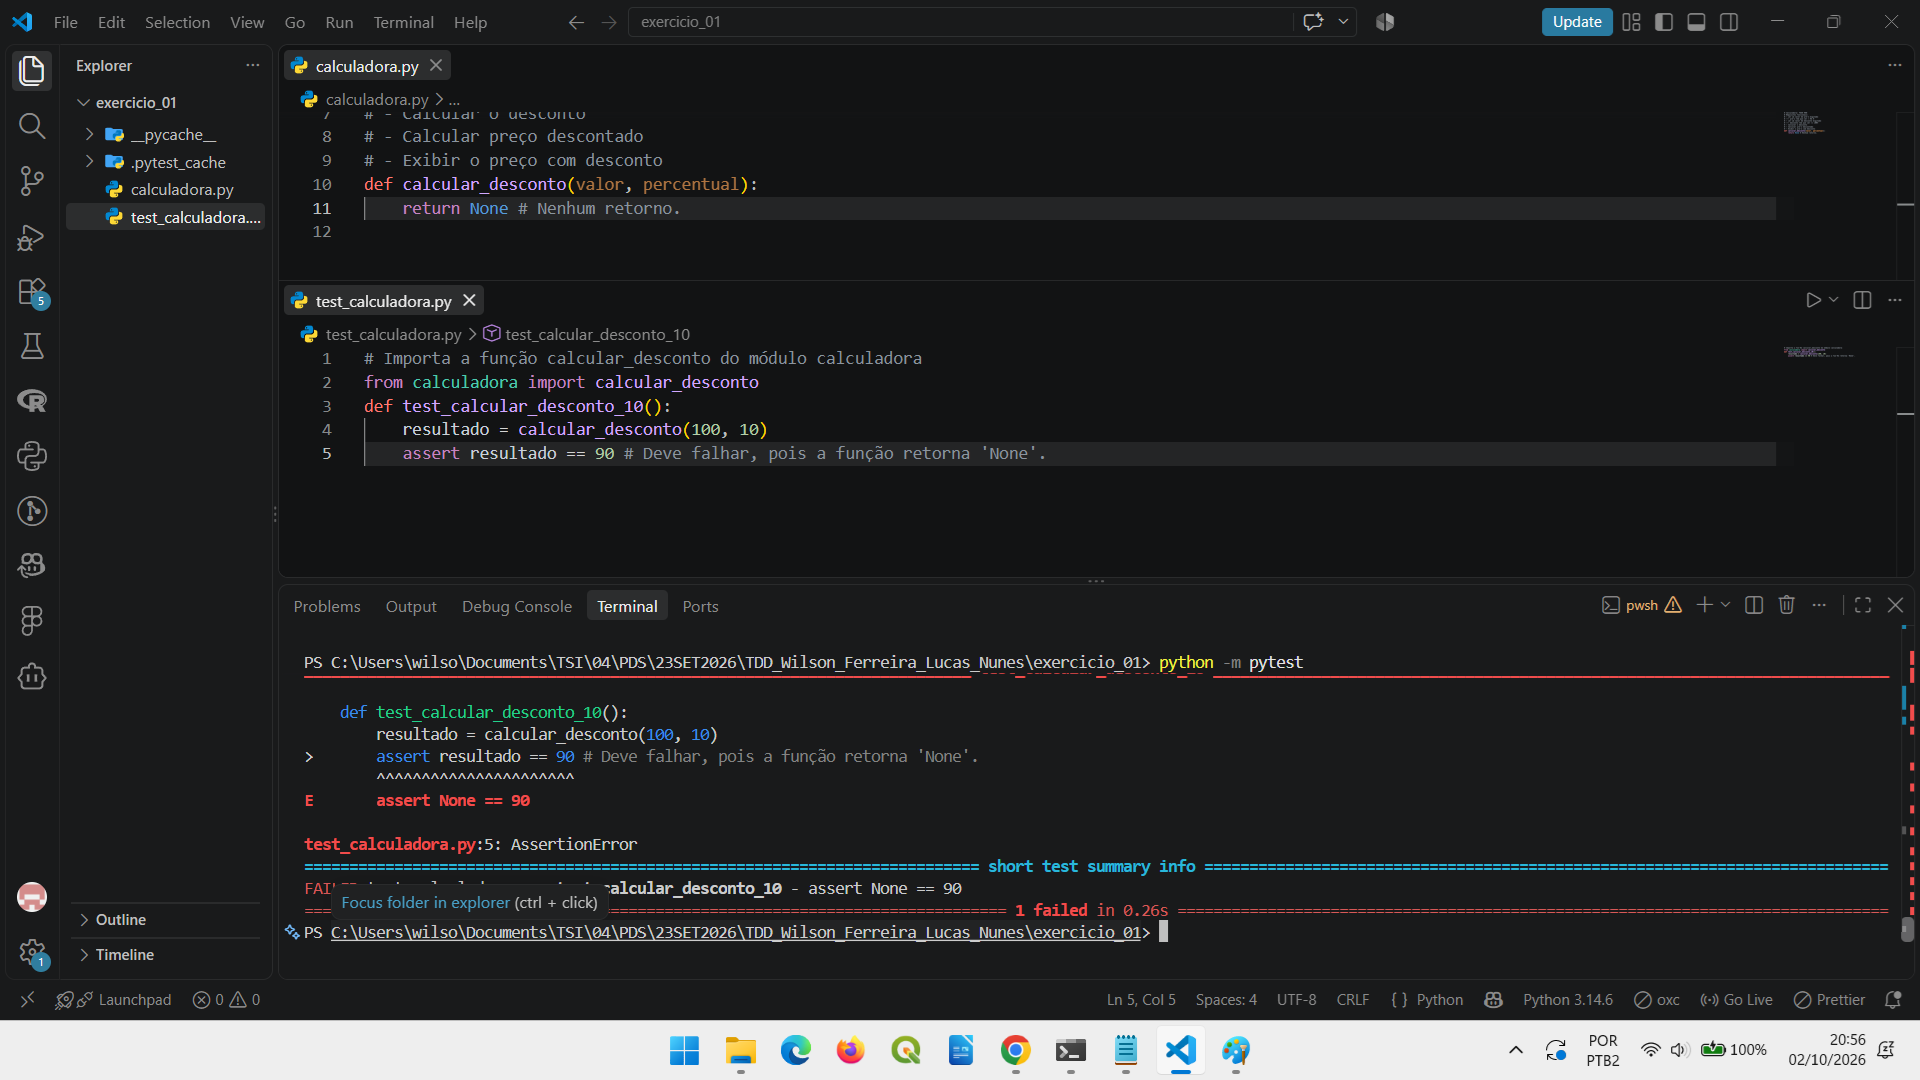
\includegraphics[width=0.92\textwidth]{ex01_red.png}
        \caption{Evidência da fase RED: falha de asserção no Pytest.}
        \label{fig:ex01_red}
    \end{figure}

    \item \textbf{Como você fez o teste passar?}
    
    A fórmula matemática mínima necessária foi implmentada em \texttt{calculadora.py}: o cálculo do valor final descontado através da expressão \texttt{valor * (1 - percentual / 100)}, satisfazendo a asserção e fazendo a execução verde no \textit{Pytest} (fase GREEN).

    \begin{figure}[htbp]
        \centering
        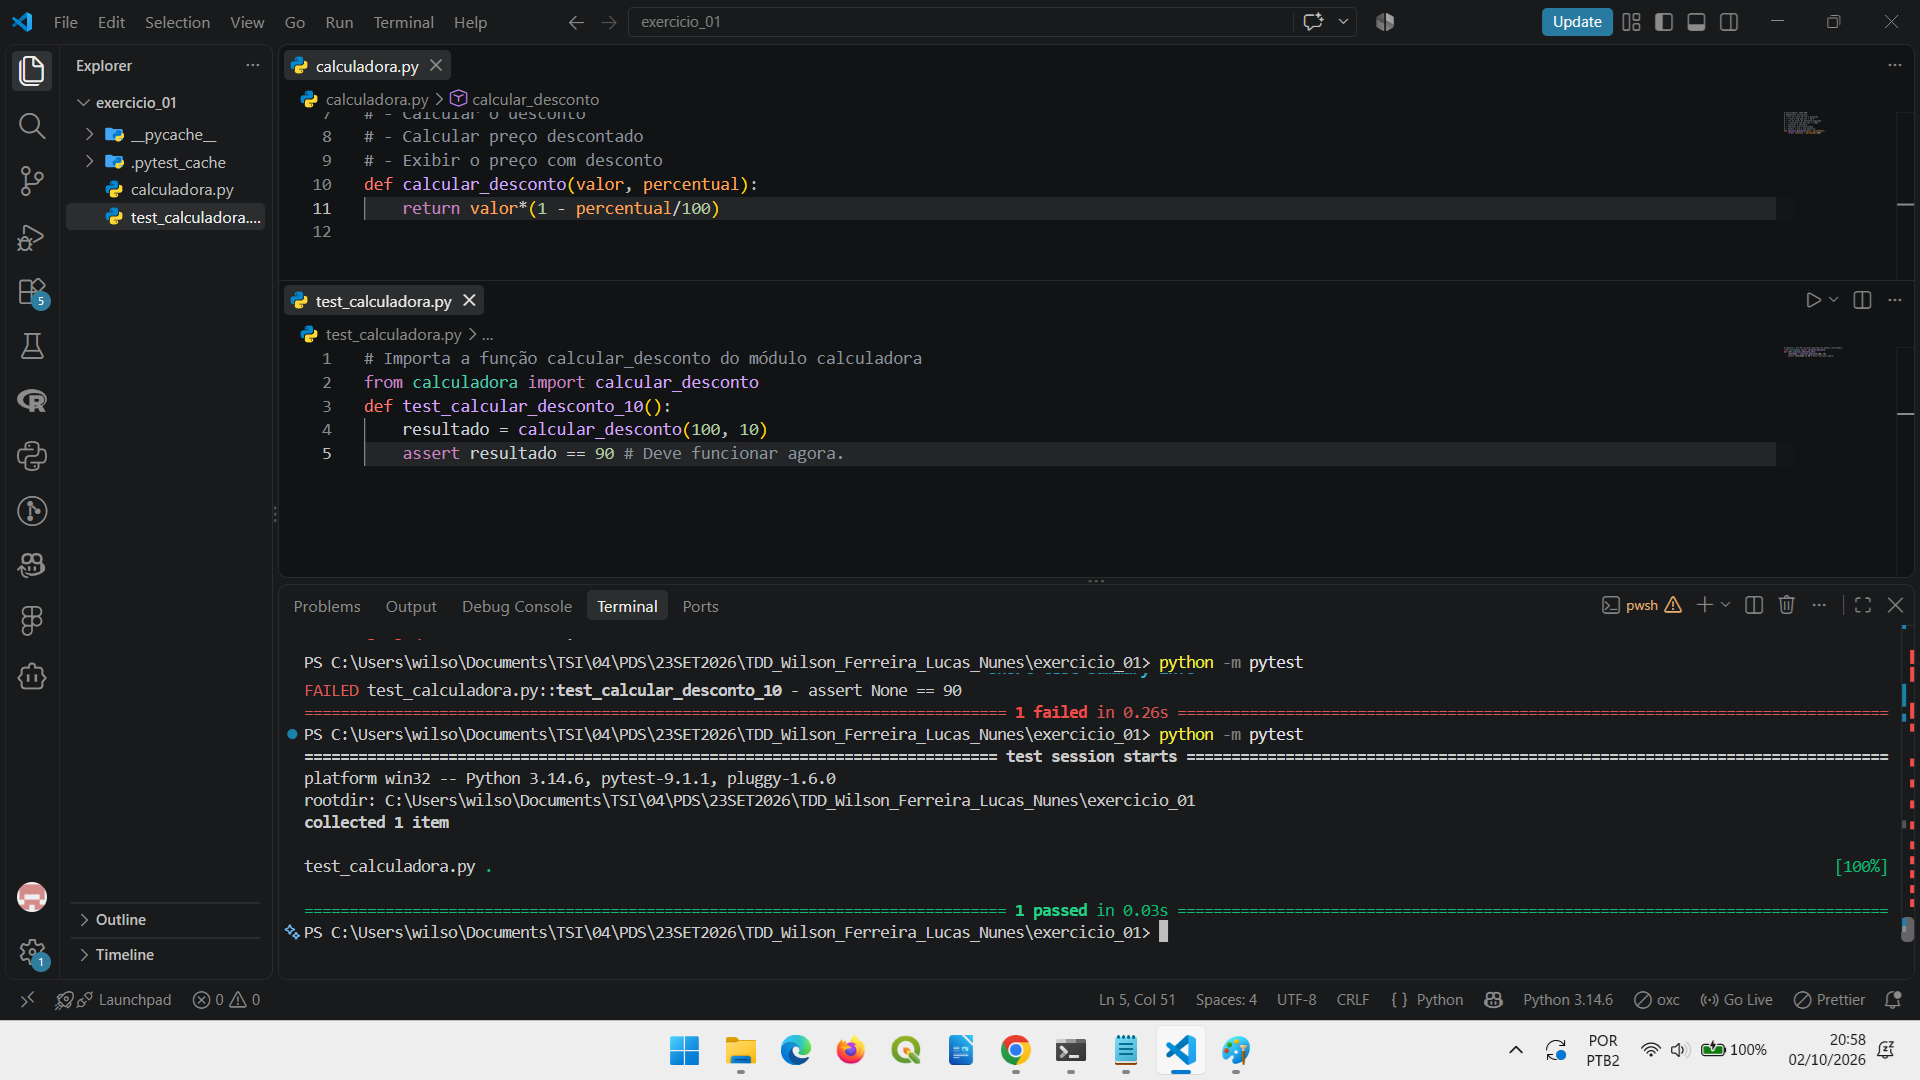
\includegraphics[width=0.92\textwidth]{ex01_green.png}
        \caption{Evidência da fase GREEN: teste obrigatório aprovado.}
        \label{fig:ex01_green}
    \end{figure}

    \item \textbf{O que foi alterado durante a refatoração?}
    
    Na fase REFACTOR, o conjunto de testes foi expandido para cobrir todos os cenários obrigatórios (20\%, 0\% e 100\%) da questão e os casos do desafio adicional (preço negativo e desconto superior a 100\%). Em \texttt{calculadora.py}, foram adicionadas condições de guarda com lançamento de exceções  (\texttt{raise ValueError}), validadas via \texttt{pytest.raises(ValueError)}, confirmando  os 6 testes passando normalmente.

    \begin{figure}[htbp]
        \centering
        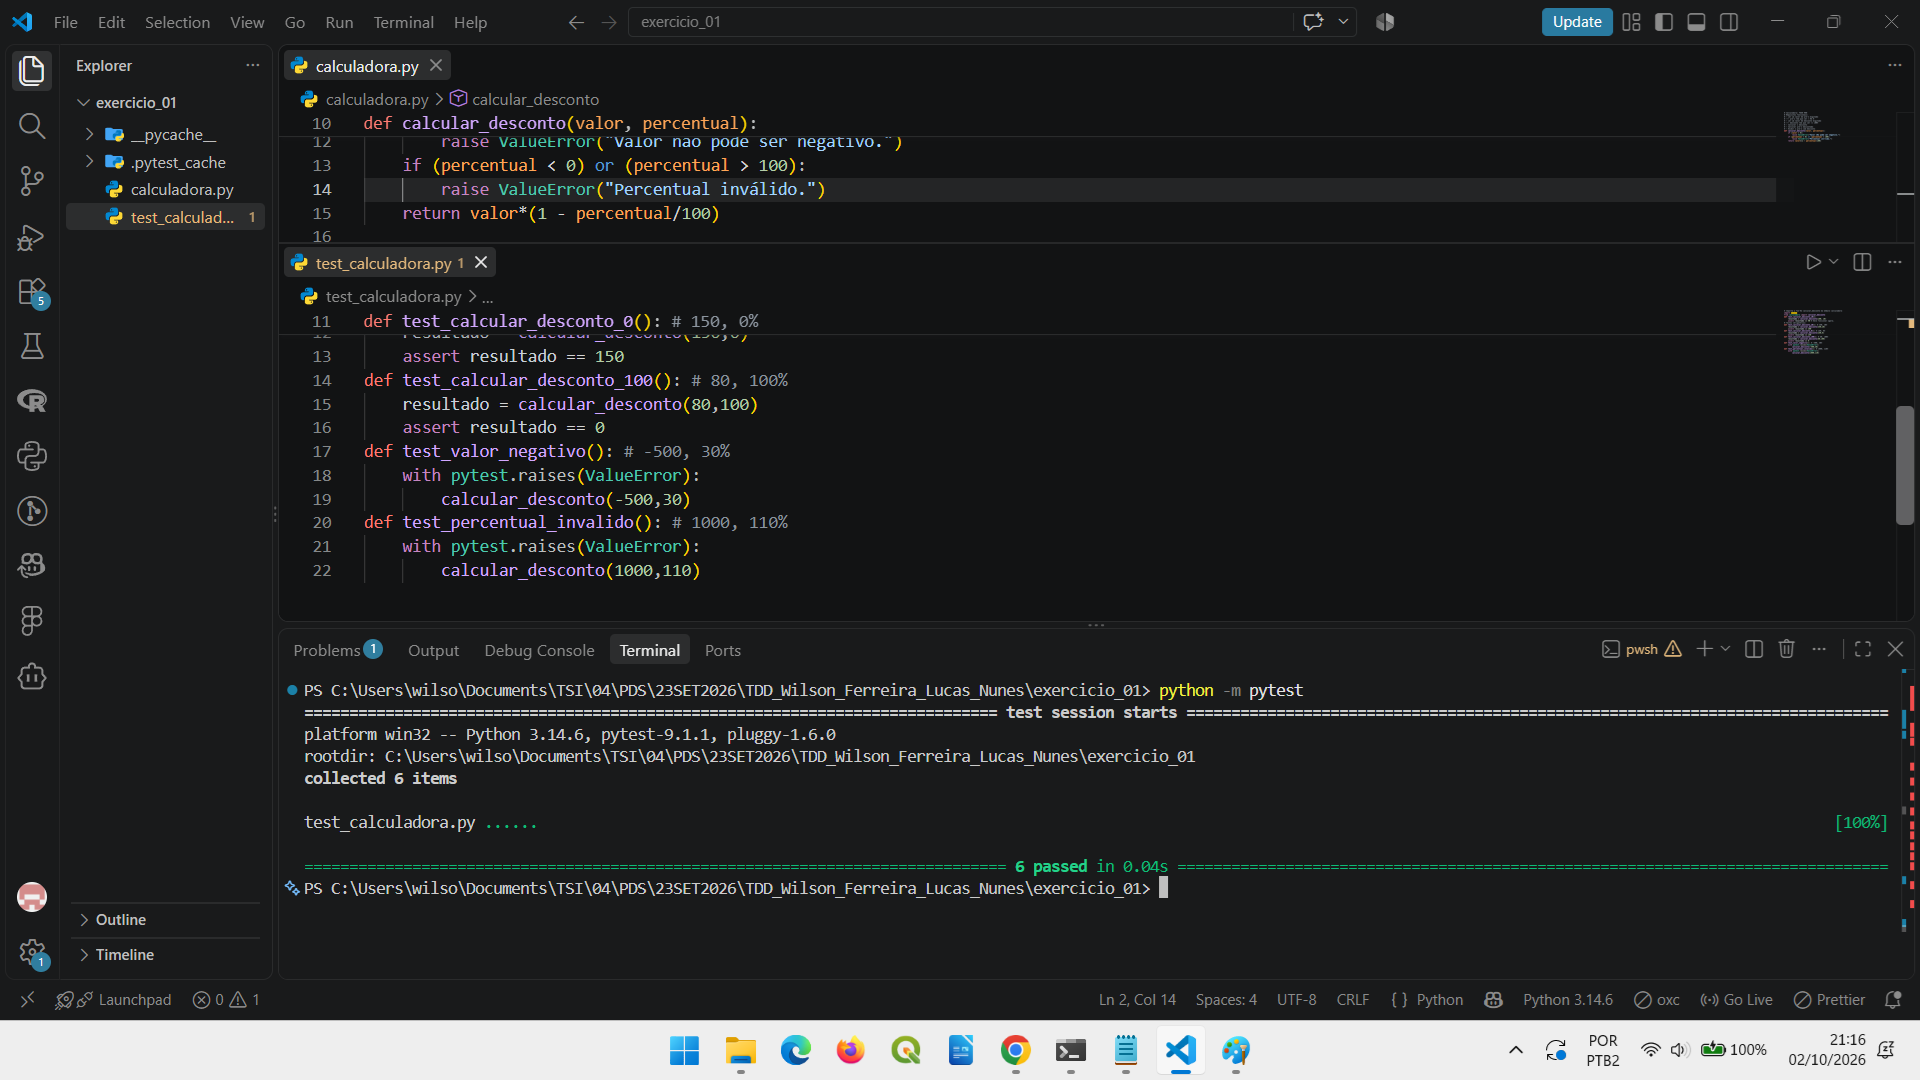
\includegraphics[width=0.92\textwidth]{ex01_refactor.png}
        \caption{Evidência da fase REFACTOR: 6 testes aprovados.}
        \label{fig:ex01_refactor}
    \end{figure}
\end{enumerate}
\newpage

\section*{Exercício 2: Sistema de Classificação de Notas}

\begin{enumerate}
    \item \textbf{Quais testes foram criados?}
    
    Foram concebidos e executados 7 testes unitários automatizados com recurso ao \textit{Pytest} no módulo \texttt{test\_notas.py}, cobrindo todos os cenários obrigatórios e os casos de exceção:
    \begin{itemize}
        \item \texttt{test\_nota\_quatro\_reprovado()}: valida se a nota $4$ retorna a classificação ``Reprovado''.
        \item \texttt{test\_nota\_cinco\_recuperacao()}: valida o limite inferior da faixa de recuperação com a nota $5$.
        \item \texttt{test\_nota\_seis\_nove\_recuperacao()}: valida o limite superior da faixa de recuperação através da nota de fronteira $6{,}9$.
        \item \texttt{test\_nota\_sete\_nove\_aprovado()}:\\ valida o limiar de aprovação através da nota $7$.
        \item \texttt{test\_nota\_dez\_aprovado()}: valida a pontuação máxima da escala com a nota $10$.
        \item \texttt{test\_nota\_negativa\_invalida()}: valida o lançamento de exceção para valores estritamente negativos (ex.: $-15$).
        \item \texttt{test\_nota\_maior\_que\_dez\_invalida()}: \\ valida o lançamento de exceção para valores que excedem a escala (ex.: $15$).
    \end{itemize}

    \begin{figure}[htbp]
        \centering
        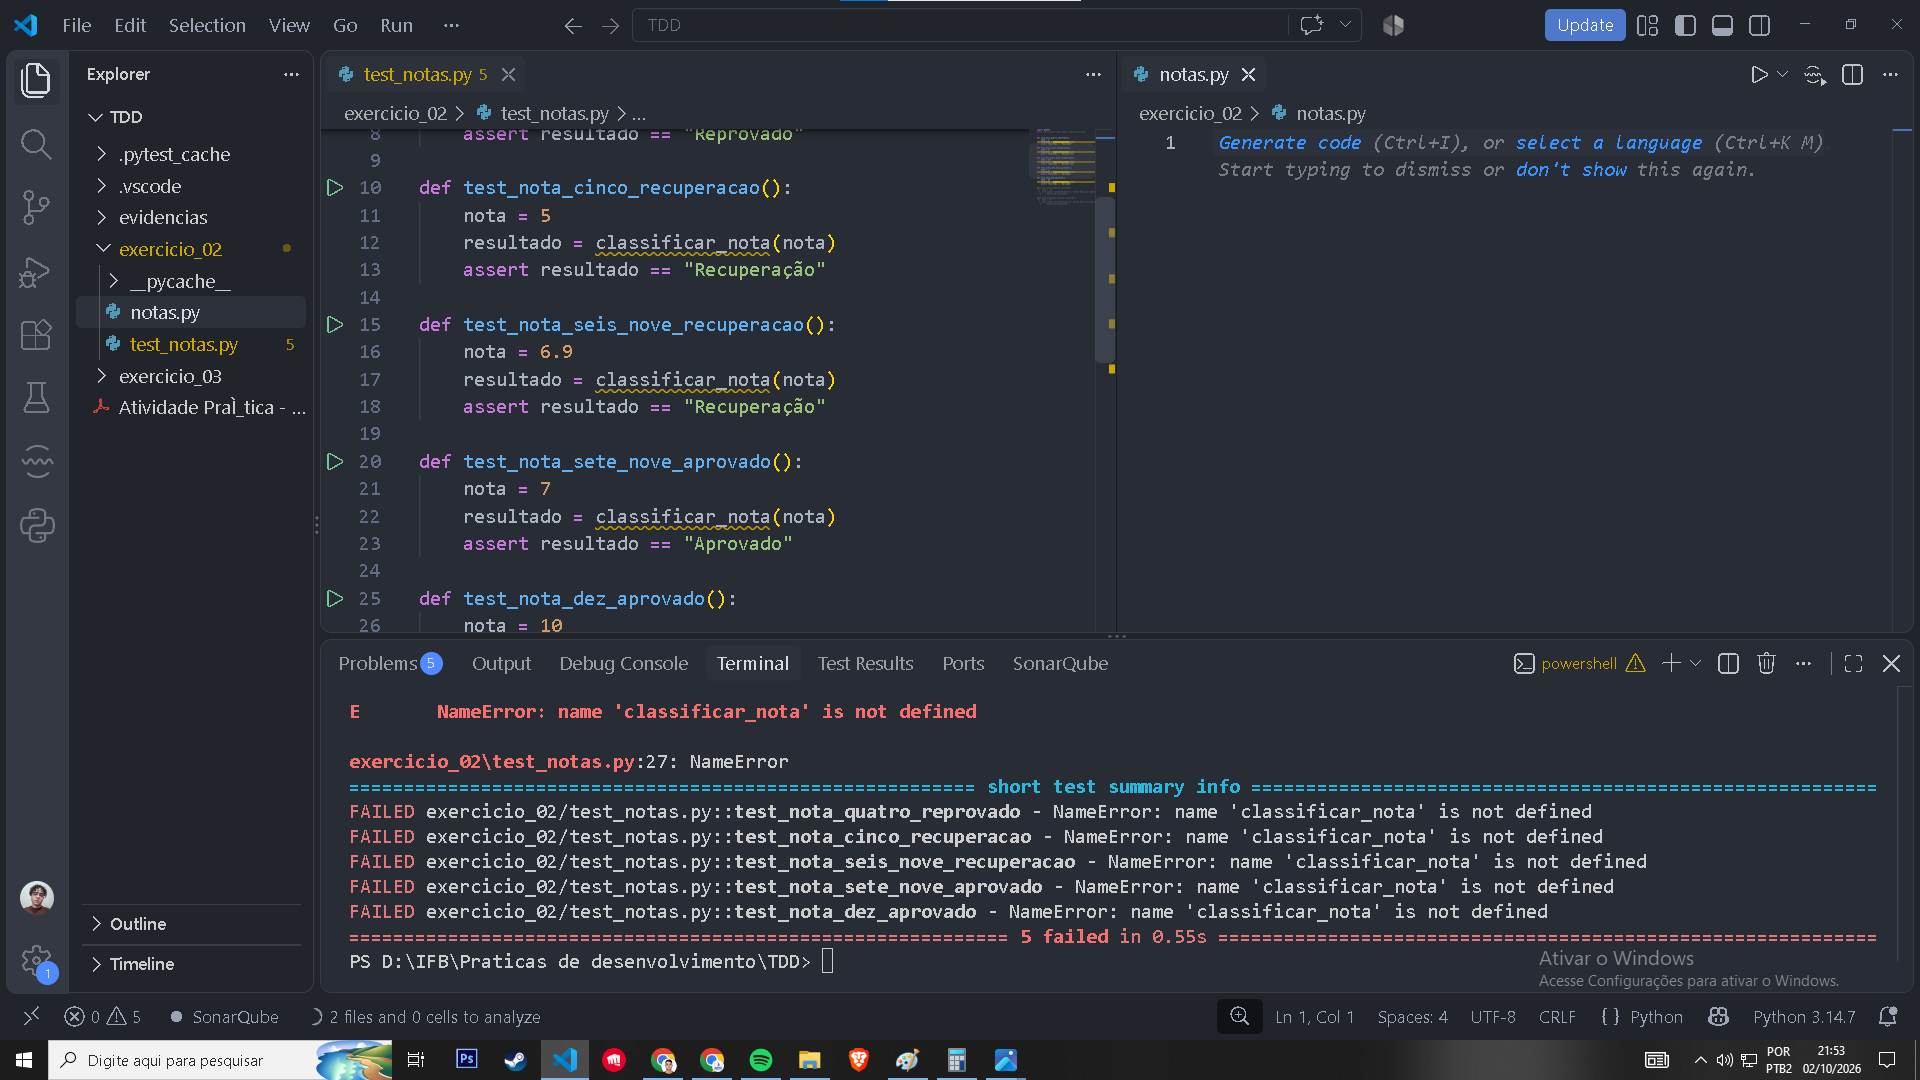
\includegraphics[width=0.92\textwidth]{ex02_red.png}
        \caption{Evidência da fase RED: falha inicial no Pytest (\textit{NameError}) antes da definição da função no módulo.}
        \label{fig:ex02_red}
    \end{figure}

    \item \textbf{Qual caso de teste apresentou maior dificuldade?}
    
    A maior exigência técnica residiu na validação dos casos de fronteira (\textit{boundary value analysis}), com particular destaque para o limite superior da faixa de recuperação na nota $6{,}9$ em transição direta para a nota $7$ (aprovação). Foi necessário garantir que a lógica condicional em \texttt{notas.py} operasse com operadores relacionais adequados (\texttt{nota < 7}), evitando desvios com números decimais. Paralelamente, a estruturação dos testes para verificar o disparo e a captura correta de exceções demandou o uso rigoroso do gestor de contexto \texttt{pytest.raises}.

    \begin{figure}[htbp]
        \centering
        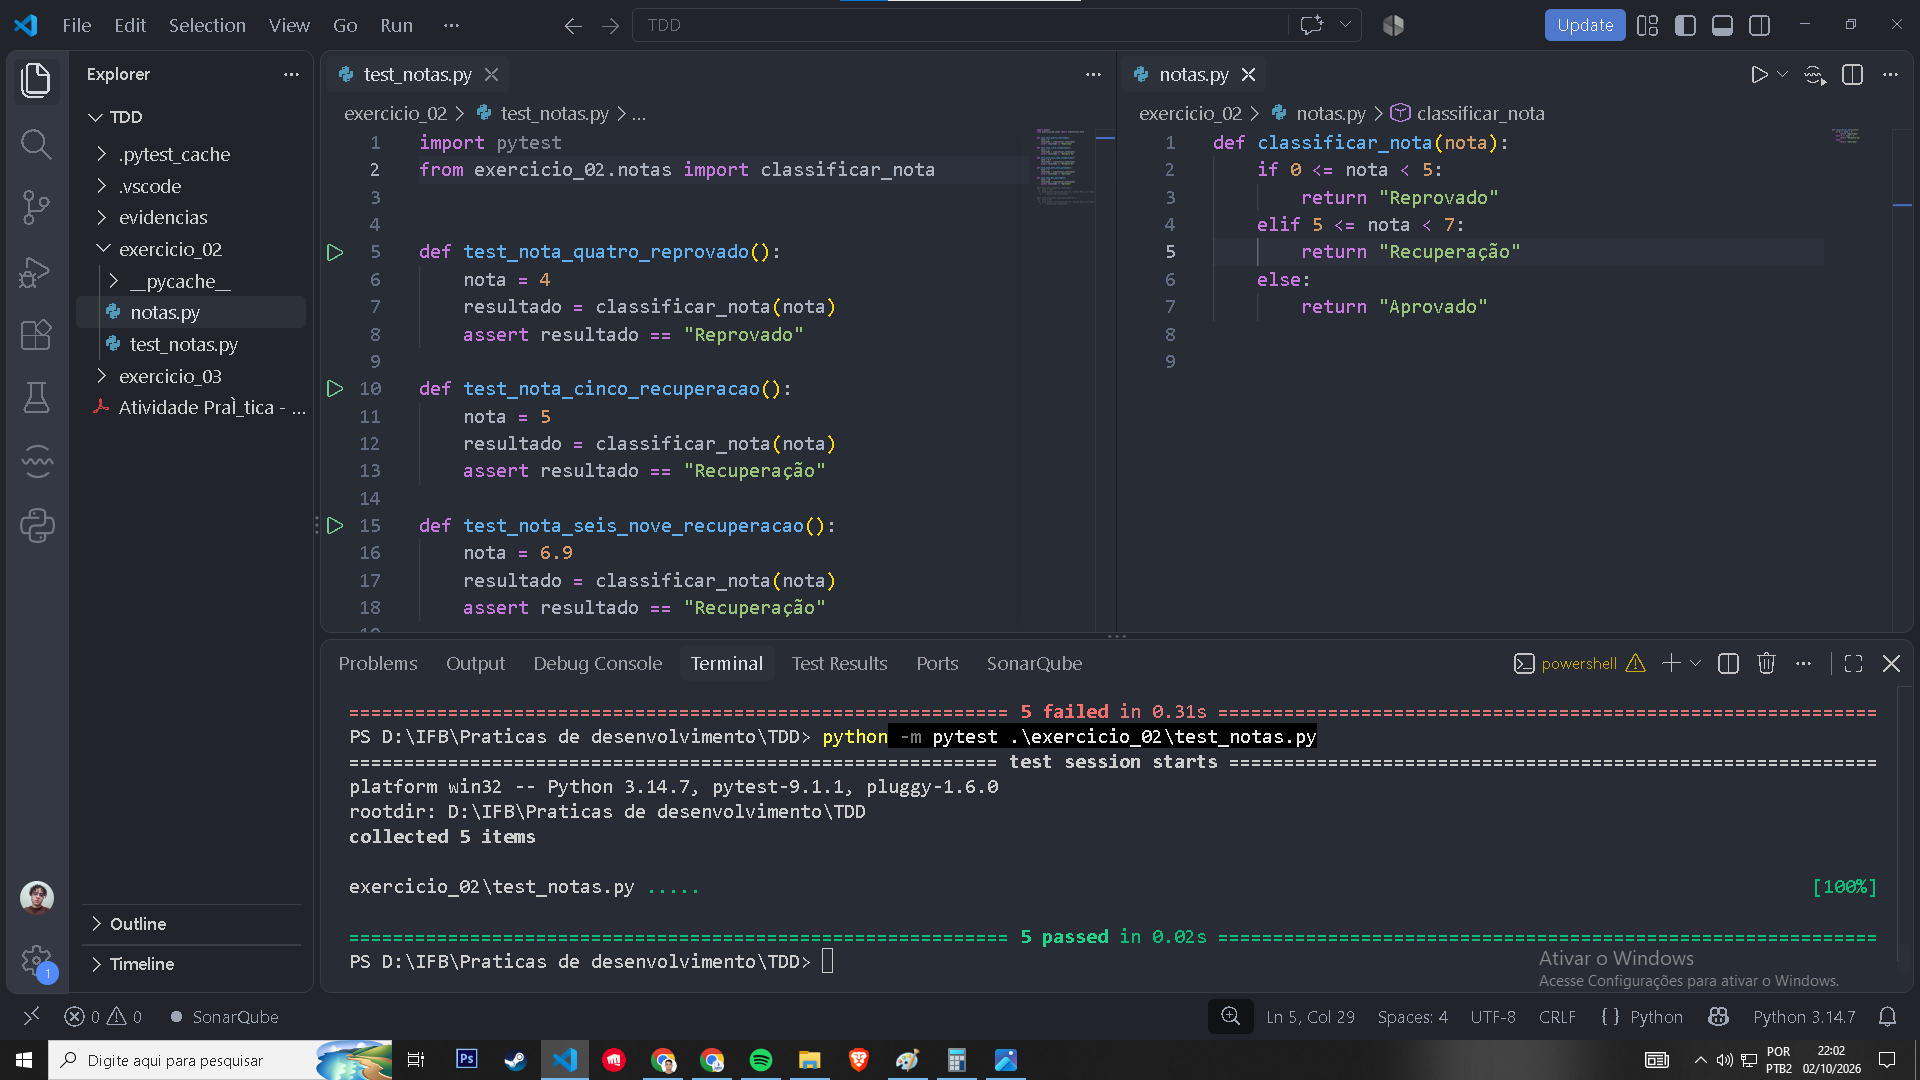
\includegraphics[width=0.92\textwidth]{ex02_green.png}
        \caption{Evidência da fase GREEN: bateria com os 5 casos de teste de classificação obrigatórios aprovados.}
        \label{fig:ex02_green}
    \end{figure}

    \item \textbf{Como você tratou notas inválidas?}
    
    O tratamento de entradas inválidas (valores estritamente inferiores a zero ou superiores a dez) foi feito via lançamento explícito da exceção \texttt{ValueError} seguida da descrição \texttt{"Nota inválida"}. Seguindo o fluxo TDD, foram criados previamente os testes com \texttt{with pytest.raises(ValueError, match="Nota inválida")}, observada a sua falha e, a seguir, criada a cláusula de guarda no módulo \texttt{notas.py}. A execução confirmou a passagem integral da suíte de testes completa.

    \begin{figure}[htbp]
        \centering
        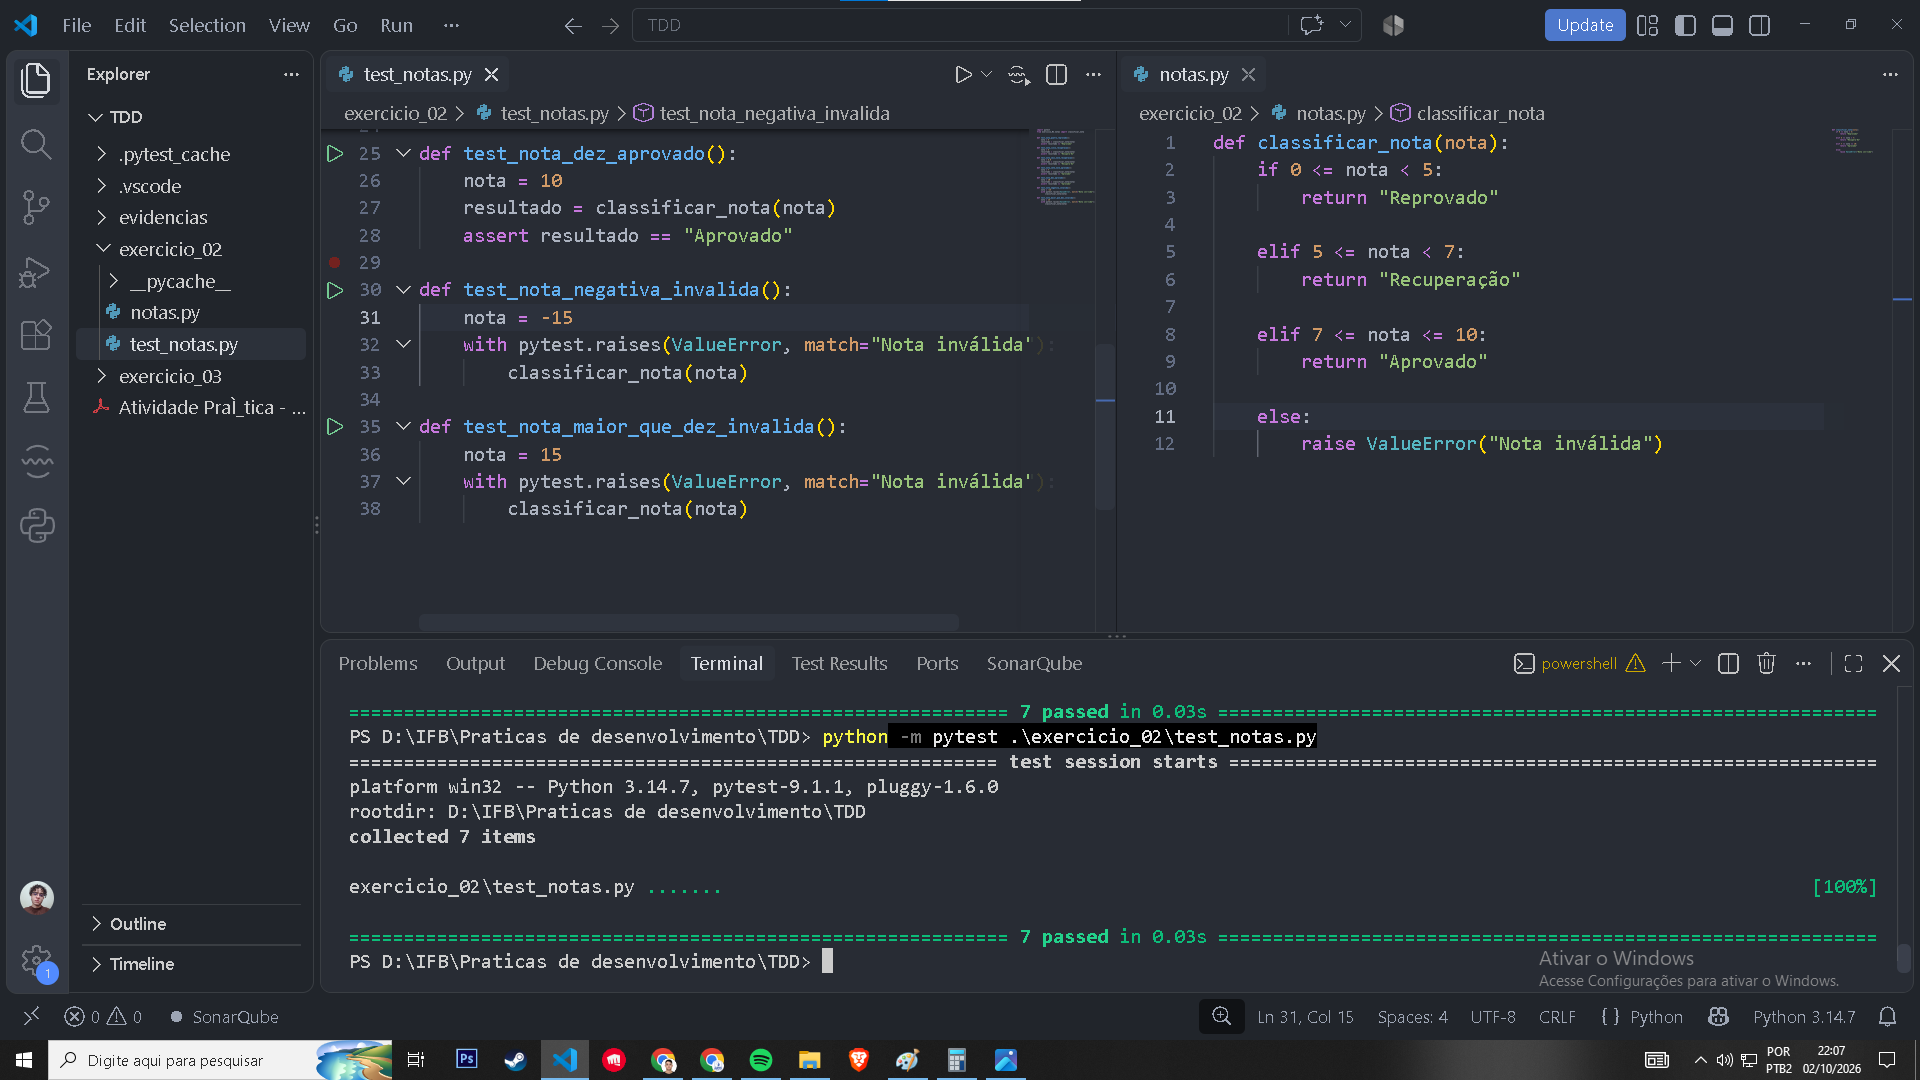
\includegraphics[width=0.92\textwidth]{ex02_refactor.png}
        \caption{Evidência da fase REFACTOR: suíte completa com os 7 testes executados com sucesso no Pytest.}
        \label{fig:ex02_refactor}
    \end{figure}
\end{enumerate}
\newpage

\section*{Exercício 3: Carrinho de Compras}

\begin{figure}[htbp]
    \centering
    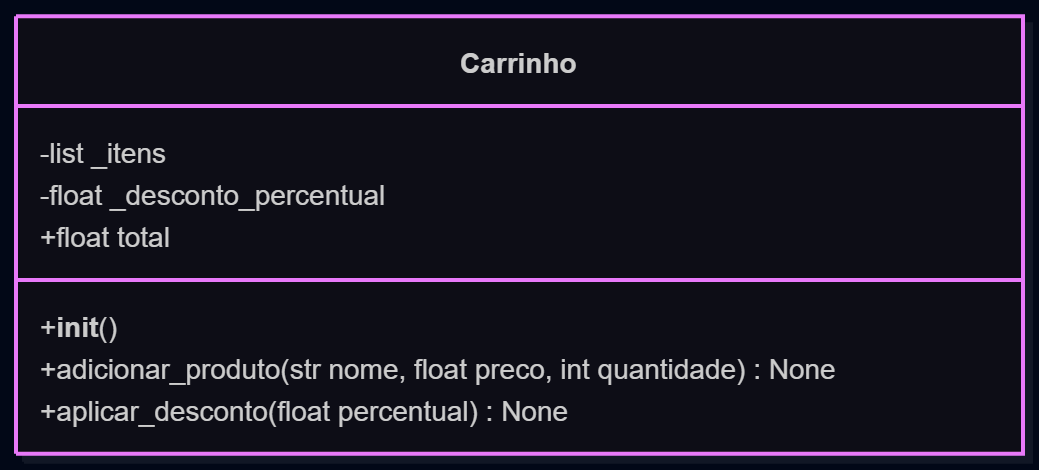
\includegraphics[width=0.65\textwidth]{carrinho_uml.png}
    \caption{Modelagem de classes UML da entidade Carrinho.}
    \label{fig:carrinho_uml_claro}
\end{figure}

\begin{enumerate}
    \item \textbf{Quais funcionalidades foram implementadas?}
    
    Foi desenvolvida a classe \texttt{Carrinho} com suporte completo às seguintes operações de negócio:
    \begin{itemize}
        \item Inicialização do estado interno com uma lista de itens vazia e percentual de desconto zerado.
        \item Adição de itens unitários ou múltiplos informando nome, preço e parâmetro opcional de quantidade (com valor padrão unitário).
        \item Validação defensiva de entrada: rejeição de quantidade menor ou igual a zero com lançamento da exceção \\ \texttt{ValueError("Quantidade inválida")}.
        \item Aplicação de desconto percentual acumulável sobre o valor total do carrinho.
        \item Cálculo dinâmico do montante total via método \texttt{total()}, que percorre os itens acumulando os subtotais e aplicando o abatimento percentual configurado.
    \end{itemize}

    \item \textbf{Quais testes foram criados?}
    
    No módulo \texttt{test\_carrinho.py}, foram implementados 6 casos de teste automatizados com o \textit{Pytest} para validar as regras obrigatórias:
    \begin{itemize}
        \item \texttt{teste\_carrinho\_vazio()}: confirma que uma nova instância do carrinho inicia com total igual a 0.
        \item \texttt{teste\_produto\_100\_total\_100()}: verifica a inserção de um único produto (Mouse de R\$ 100,00) totalizando R\$ 100,00.
        \item \texttt{teste\_dois\_produtos\_total\_250()}: valida a inserção cumulativa de dois produtos distintos (Mouse de R\$ 100,00 e Teclado de R\$ 150,00), totalizando R\$ 250,00.
        \item \texttt{teste\_produtos\_com\_quantidade\_total\_300()}: \\ testa o parâmetro explícito de quantidade (Mouse de R\$ 100,00 com quantidade 3), resultando no total de R\$ 300,00.
        \item \texttt{teste\_total\_500\_10\_porcento\_desconto()}: valida o abatimento percentual de 10\% sobre um carrinho de R\$ 500,00, confirmando o total final de R\$ 450,00.
        \item \texttt{teste\_quantidade\_invalida()}: valida o fluxo de exceção ao tentar inserir um produto com quantidade igual a 0, assegurando o disparo de \texttt{ValueError} via \texttt{pytest.raises}.
    \end{itemize}

    \begin{figure}[htbp]
        \centering
        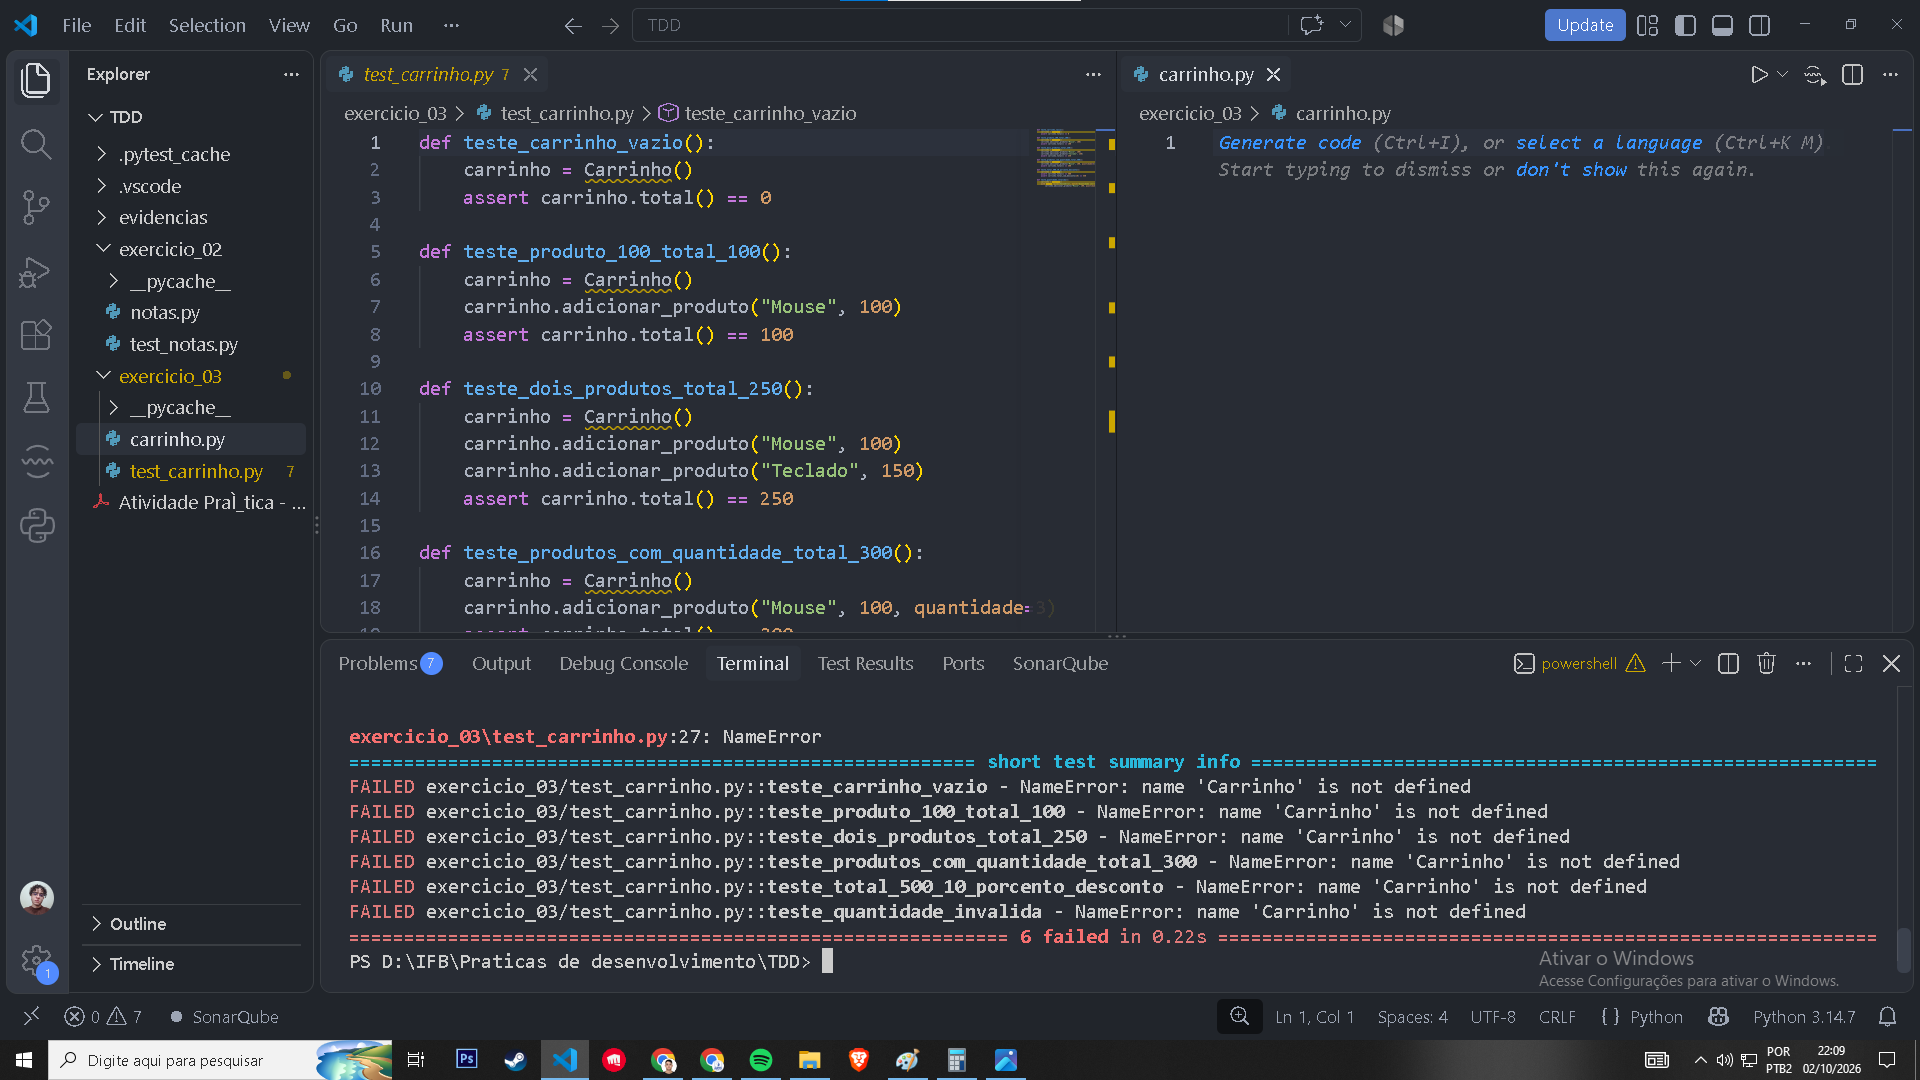
\includegraphics[width=0.92\textwidth]{ex03_red.png}
        \caption{Evidência da fase RED: execução prévia dos testes acusando NameError pela ausência da classe.}
        \label{fig:ex03_red}
    \end{figure}

    \vspace{1.0cm}
    
    \item \textbf{Qual foi a principal dificuldade encontrada durante o desenvolvimento?}
    
    A principal dificuldade foi a utilização do Python para a definição de classe. Questões como a obrigatoriedade da referência explícita \texttt{self} nos métodos de instância, o controle estrito de indentação de blocos e a manipulação de estruturas de dados dinâmicas (dicionários e listas por compreensão no cálculo do somatório) exigiram atenção. Além disso, compreender o ciclo do TDD na modelagem de classes — garantindo que a interface pública dos métodos fosse planejada primeiro a partir do teste unitário antes de qualquer definição da estrutura interna da classe — exigiu uma mudança de raciocínio em relação ao desenvolvimento tradicional.

    \begin{figure}[htbp]
        \centering
        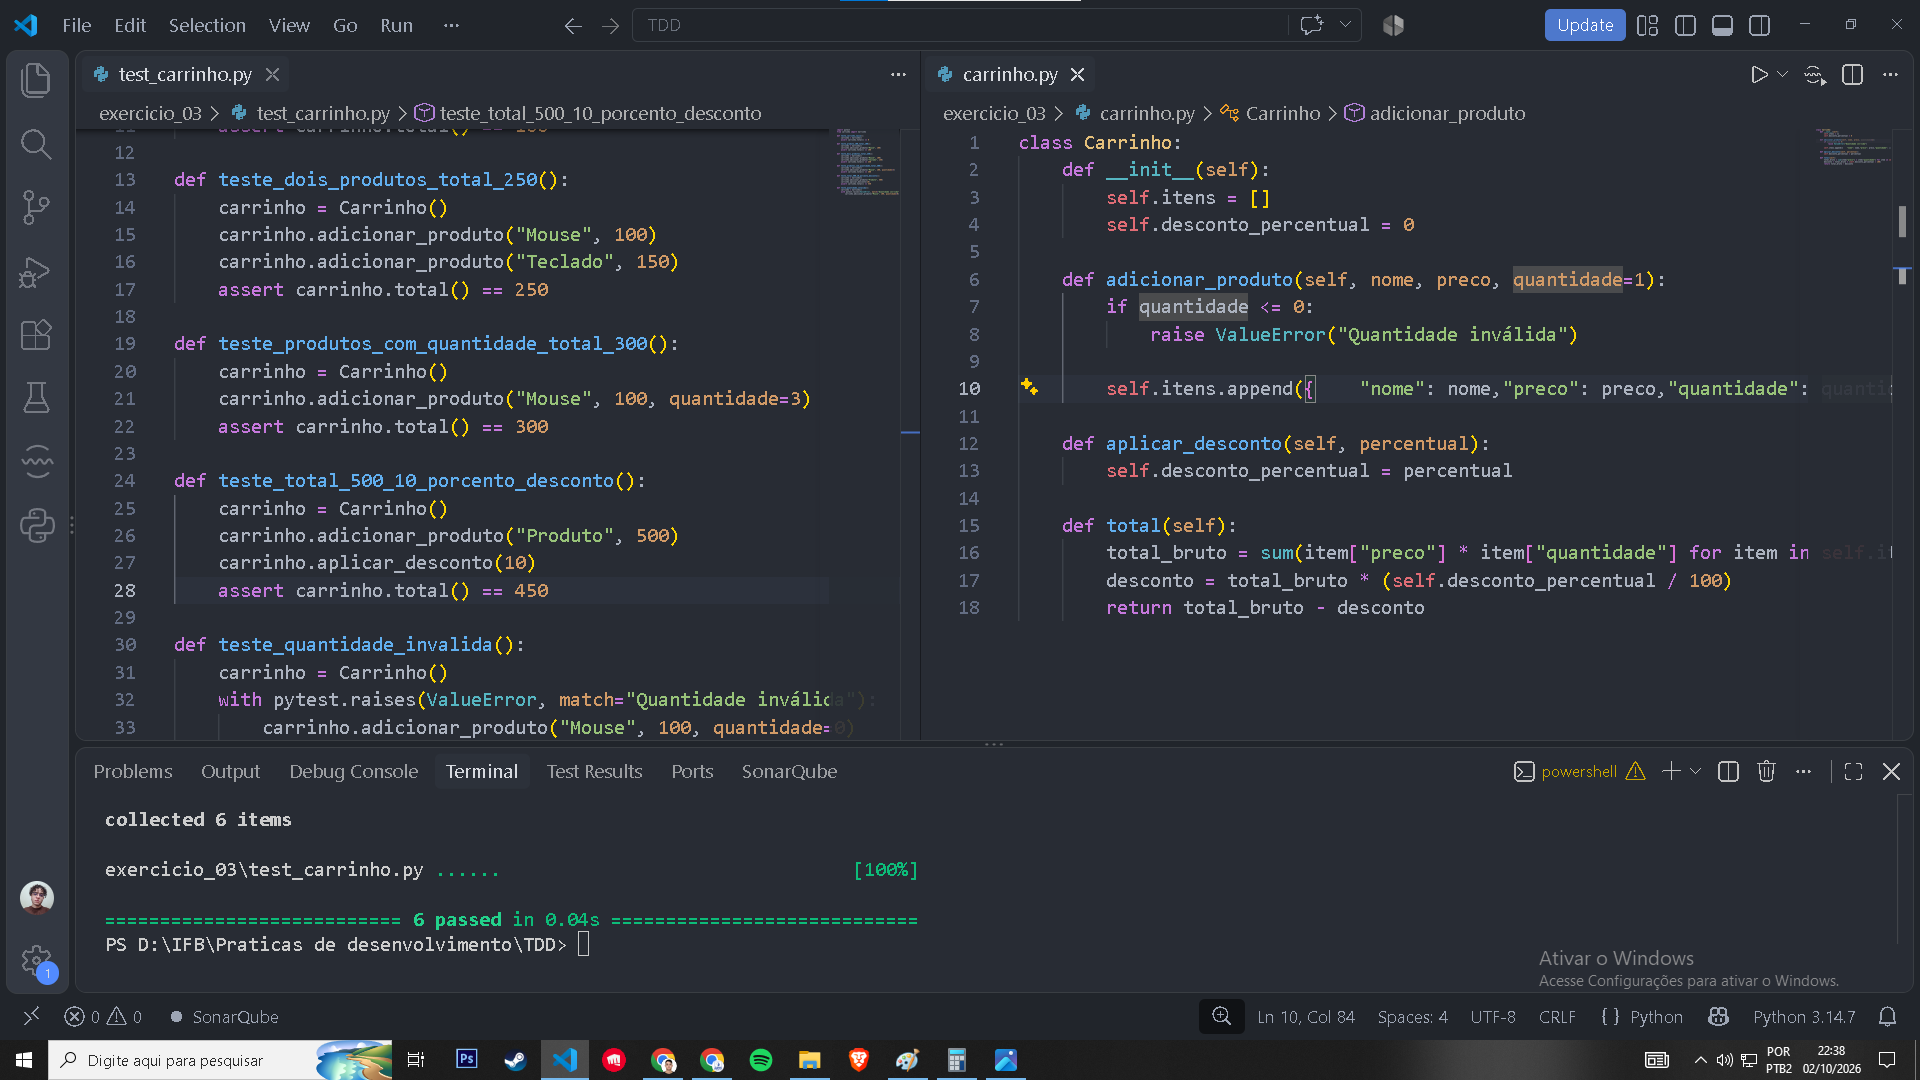
\includegraphics[width=0.92\textwidth]{ex03_green.png}
        \caption{Evidência da fase GREEN: implementação da classe satisfazendo todos os 6 testes no Pytest.}
        \label{fig:ex03_green}
    \end{figure}

    \begin{figure}[htbp]
        \centering
        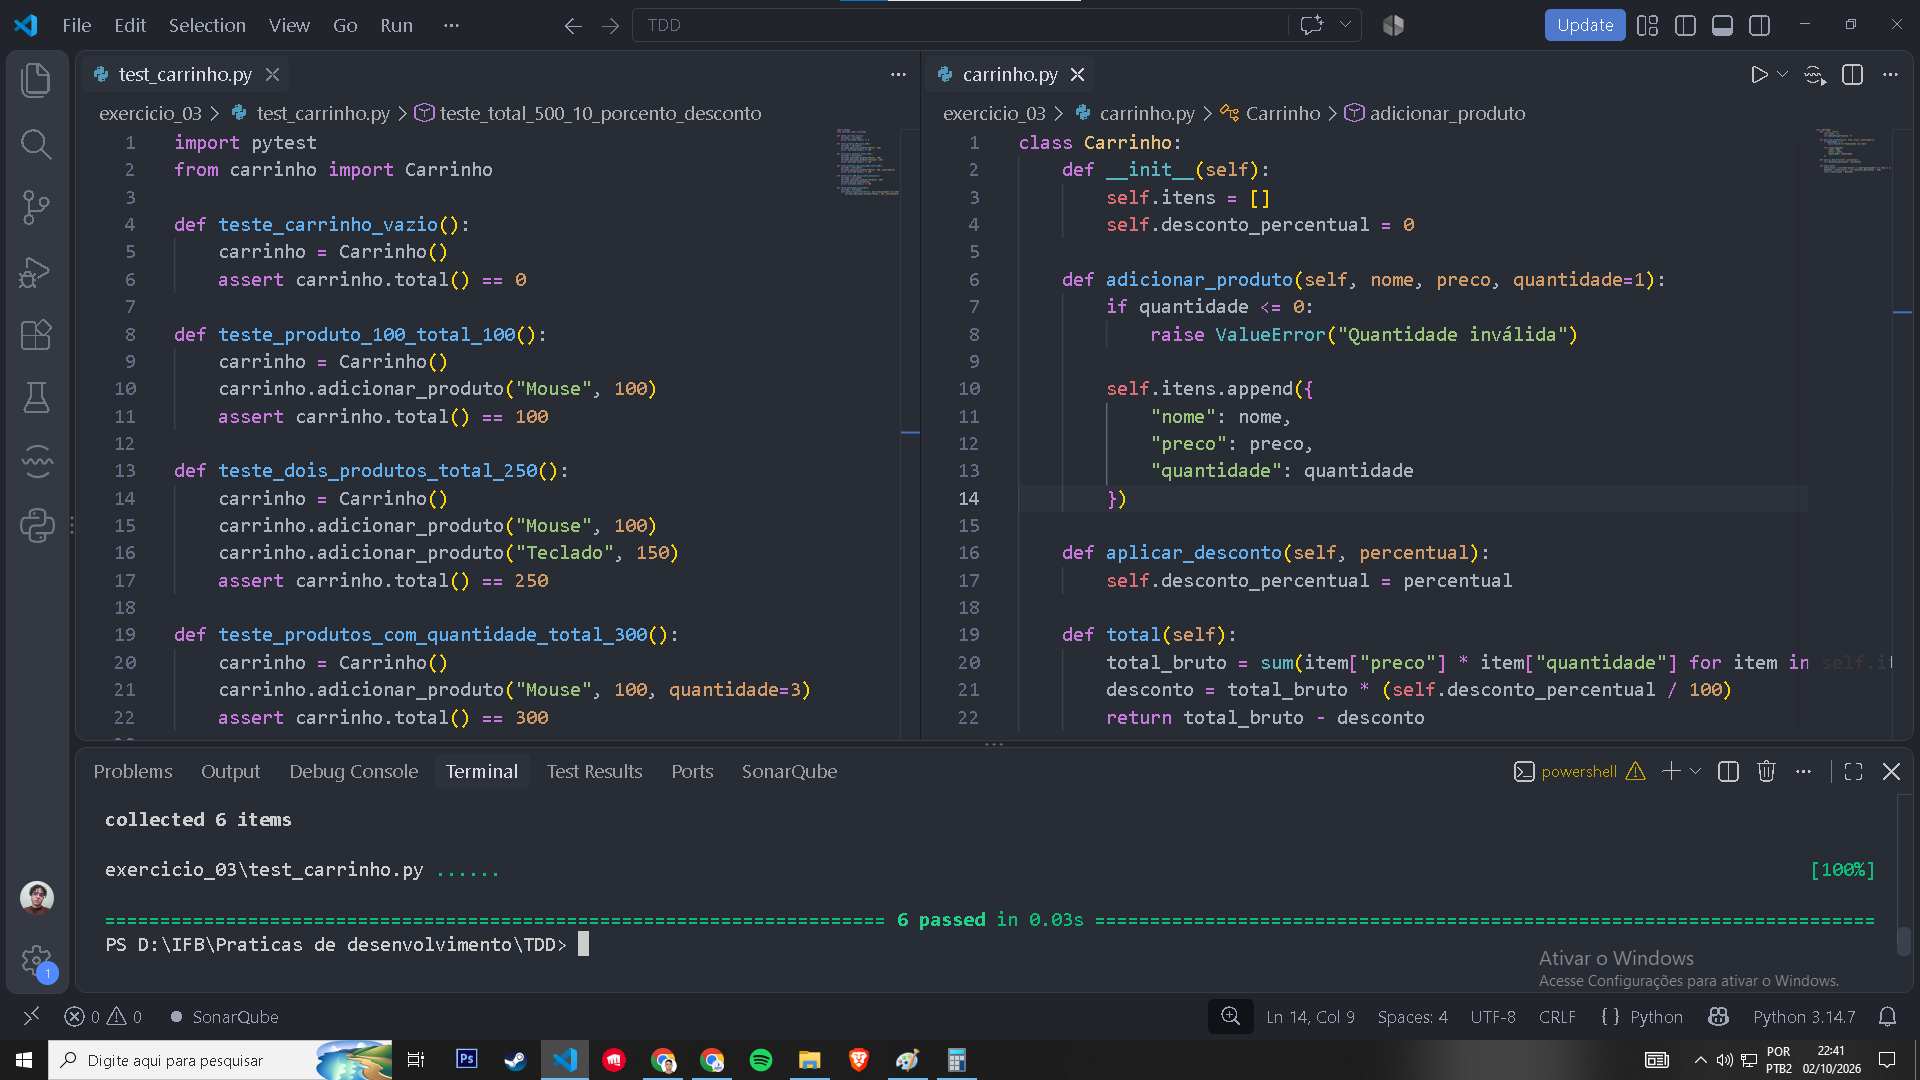
\includegraphics[width=0.92\textwidth]{ex03_refactor.png}
        \caption{Evidência da fase REFACTOR: suíte integral com os 6 testes passando com código consolidado.}
        \label{fig:ex03_refactor}
    \end{figure}
\end{enumerate}
\newpage

\Large{\textbf{Reflexão final:}}
\begin{itemize}
    \item Explique, com suas próprias palavras, o que significa RED → GREEN → REFACTOR.
    
    Prática de desenvolvimento de sistema onde primeiro se criam os testes, antes do código funcional, com a intenção de que não passem (RED), logo após isso, desenvolve-se o código mínimo para que os testes passem (Green) e depois se melhora o código em organização e legibilidade, por exemplo(Refactor).

    \item Qual é a principal diferença entre desenvolver primeiro o código e depois criar os testes
e utilizar TDD?
    
    Escrever os testes antes cria uma noção prévia do que cada método deve fazer e as limitações a considerar, incluindo exceções e tratamento de erros.

\end{itemize}

\end{document}
